\documentclass[11pt]{article}
\usepackage{fullpage}
\usepackage{amsmath}
\usepackage{amssymb}
\usepackage{gensymb}
\usepackage{graphicx}
\usepackage{cancel}
\usepackage{hyperref}
\usepackage{tikz}
\usepackage{verbatim}
\usepackage{listings}
\usepackage{forest}
\hypersetup{
    colorlinks,
    citecolor=black,
    filecolor=black,
    linkcolor=blue,
    urlcolor=blue
}

\lstset{language=C++,
    basicstyle=\ttfamily,
    keywordstyle=\color{blue}\ttfamily,
    stringstyle=\color{red}\ttfamily,
    commentstyle=\color{gray}\ttfamily,
    morecomment=[l][\color{magenta}]{\#},
    showstringspaces=false
}

\usetikzlibrary{calc, shapes.geometric, arrows}

\tikzstyle{redrect} = [rectangle, rounded corners, minimum width=3cm, 
    minimum height=1cm,text centered, draw=black, fill=red!30]
    
\tikzstyle{bluerect} = [rectangle, rounded corners, minimum width=3cm, 
    minimum height=1cm,text centered, draw=black, fill=blue!30]

\tikzstyle{orangerect} = [rectangle, rounded corners, minimum width=3cm, 
    minimum height=1cm,text centered, draw=black, fill=orange!30]

\tikzstyle{arrow} = [thick,->,>=stealth]


\title{\vspace{10em}ME 759 Final Project Report \\ Default Project 1: Distributed Task Library}
\author{William Jen \\ University of Wisconsin-Madison}
\date{December 2017}

\begin{document}
    \maketitle

    \pagebreak
    
    \section{Abstract}
        Default Project 1 defines a situation where simulating a process can be broken up into smaller sized
        tasks that can be executed in parallel, either on machine or remotely. Although MPI provides useful 
        functions to communicate and send data with other nodes, it is effectively transport-layer, meaning
        that it is up to the programmer to synchronize data and determine how to execute code in parallel.
        The Distributed Task Library aims to provide a set of classes that will allow the user to easily
        specify what code needs to be run in parallel and where. The Task class is capable of spinning off
        threads to execute code on a local machine, and the TaskManager class can create and issue work
        to MPI nodes dynamically.
        
    \tableofcontents
    \pagebreak
    
    \section{Introduction}
        Default Project 1 was described as an "OpenMP-based parallel and decoupled mechanism for
        asynchronous update of an on-going process.". In other words, a parent job $P$ may run in 
        a loop. Within that loop, it may spawn children tasks $C_1 \ldots C_n$ that can be run on either
        the same machine in a different thread or a separate machine entirely. Furthermore, these tasks may
        use GPU acceleration, so if a child task is set to run on a different machine, it must be run on a 
        machine with a GPU. Additionally, the parent task $P$ must not advance to the next iteration of the loop
        before all of its children tasks have completed. The goal of this project is to define a software framework 
        that will allow the programmer to spawn child tasks on the location of their choice (same host, new host, 
        GPU-enabled host) with the ability to wait for children tasks.
    
    \section{Design}
        The Distributed Task Library breaks this project into two parts: task running on the local machine and 
        task running on remote machines. To maximize portability, cross-platform libraries and technologies 
        were selected, such as C++11 threads, OpenMPI, and Google Protobuf. The main idea behind this library
        was to allow the programmer to specify function pointers to their code, and have the library take care of
        the rest. 

        \subsection{Creating Jobs Locally: A Simple Example}
            Creating jobs locally is very similar in concept to OpenMP tasks without macros. In other words,
            the user can spawn a task, and that task can spawn children tasks. Before the parent can complete,
            it must wait for its children to finish. 
            
            The Task class is responsible for creating and running local jobs and works by spinning off
            a thread for each job. This class is best explained via an example.
            
            \pagebreak
            \begin{lstlisting}[language=C++]
#include <iostream>
#include "Task.hpp"

void jobB(std::shared_ptr<dtl::Task> parent) 
{
    std::this_thread::sleep_for(std::chrono::seconds(1));
    std::cout << "[JobB] Task Name: " << parent->GetName() << std::endl; 
}

void jobA(std::shared_ptr<dtl::Task> parent)
{
    dtl::Task::Create("jobB-1", parent, jobB)->Run();
    dtl::Task::Create("jobB-2", parent, jobB)->Run();
    dtl::Task::Create("jobB-3", parent, jobB)->Run();
}

int main()
{
    auto t = dtl::Task::Create("jobA", nullptr, jobA);
    t->Run();
    t->Wait();
    return 0;
}
            \end{lstlisting}
                
            In this example, we create a task called jobA in the main function, and spin it off in a different
            thread. In turn, jobA creates three subtasks, each of which runs in a different thread and
            executes the jobB function. Although jobA can complete execution before its children, the parent
            task will wait for its children tasks to complete. In other words, there is an implicit barrier
            at the end of a Task that has spawned children. 
            
            The Task::Run() method is non-blocking, meaning that you can run a Task and then continue to do
            other things. You can wait for the task to complete by calling the Task::Wait() method.
            
            To be as general as possible, the Task class takes a function pointer to user code, which
            has the following signature:
                                
            \begin{lstlisting}[language=C++]
void callback(std::shared_ptr<Task> parent);
            \end{lstlisting}
                
                                
            The user callback function has a handle to the parent task, and is thus able to spawn
            children tasks by calling the Task::AddChildTask method.
            
            An example output for this code is as follows. Note that debug output within the Task class is
            included.
                
            \pagebreak
                
            \begin{verbatim}
jobA: Running...
jobB-1: Running...
jobB-2: Running...
jobB-3: Running...
jobA: waiting for children...
[JobB] Task Name: jobB-2
[JobB] Task Name: jobB-3
[JobB] Task Name: jobB-1
jobA: children complete!
jobA: children done!
            \end{verbatim}
                
            Here we can see that jobA did indeed complete faster than its children subtasks, but automatically
            synchronized with its children. If you would like to synchronize manually with a Task's children,
            you can call the Task::WaitForChildren method. This is useful if you are spawning tasks in a loop,
            and you need to have a barrier at the end of the loop rather than the end of the task method itself.
                
        \subsection{Task Class Internal Mechanism}
                Each Task object holds a user-specified name, its current state (Idle, Running, Waiting), 
                a pointer to its parent Task (may be null), the function it is to run, and finally a list of pointers
                to its children Task objects. 
                
                A conscious decision was made to minimize the number of raw pointers within the Task class, and instead
                use smart pointers to automatically handle destruction of objects. Indeed, there are no raw pointers
                at all - ensuring that objects are always automatically destroyed when they go out of scope. 
                
                
                A sample lifetime of a Task object is presented below. 
                \begin{enumerate}
                    \item Task::Create() is called with null as its parent (no parent) and will execute
                        a function $f$. A shared pointer to the created Task object is returned to the caller.

                    \item The Task::Run() method is called. A new thread is spun off, and calls the private
                        method Task::\_task\_runner\_shim(). This private method calls the user-provided
                        function $f$, which may spawn children Tasks. Children tasks are added by calling
                        Task::Create, but instead of passing nullptr for the parent Task, the parent task is passed
                        in. Recall that the parent Task object is passed in as a function parameter to the user
                        callback.
                        
                    \item After function $f$ completes, the implicit barrier is invoked: the task
                        checks if its children are complete. If the children are not done: the parent Task goes to
                        sleep through the task's children synchronization condition variable. When all of its children 
                        finish, the parent will awaken.
                        
                    \item Once all of the Task's children have completed, the current Task sets its status
                        to done. If the current Task has a parent, it notifies the parent by calling the
                        parent's CheckIfChildrenComplete() method. That method iterates through all of the children,
                        and if all children are marked as done, it notifies any thread waiting on the children
                        synchronization condition variable. This tells the parent to finish execution.
                        
                    \item The current task has now completed - the spun off thread is completed, and the thread exits.
                \end{enumerate}
            
                Graphically, the above process can be shown as follows:
            
                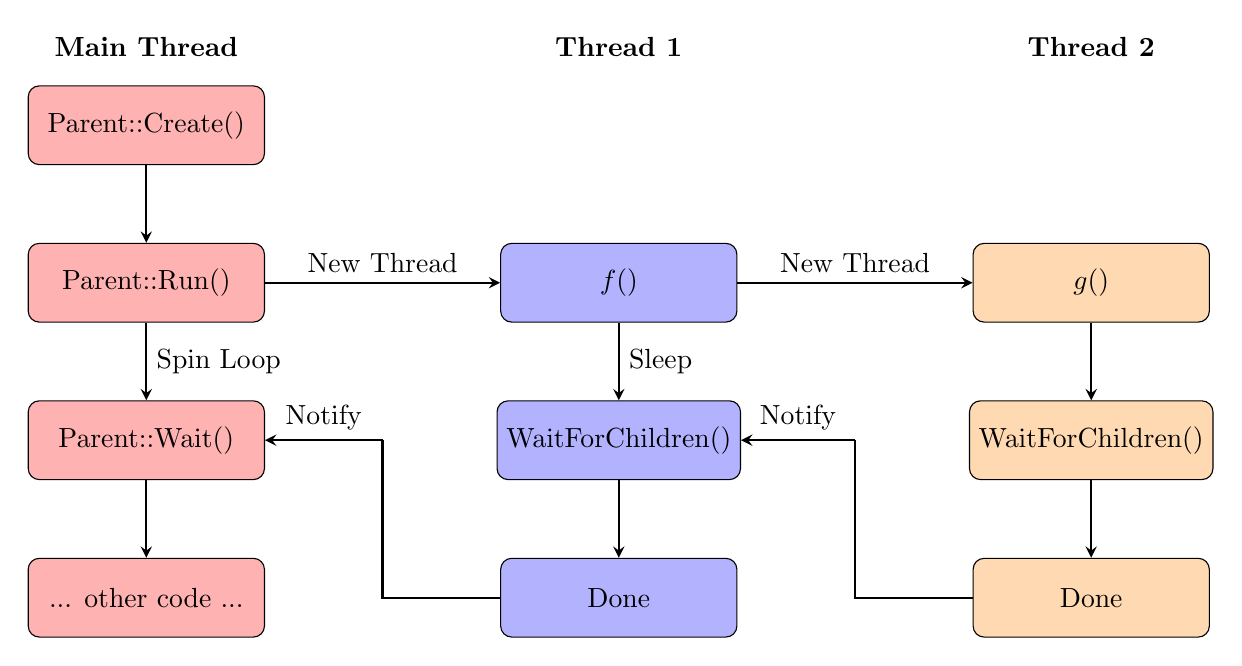
\begin{tikzpicture}[node distance=2cm]
                    % header nodes
                    \node (MainThread) {\textbf{Main Thread}};
                    \node (Thread1) [right of=MainThread, xshift=4cm] {\textbf{Thread 1}};
                    \node (Thread2) [right of=Thread1, xshift=4cm] {\textbf{Thread 2}};
                
                    % main thread nodes
                    \node (ParentCreate) [redrect, below of=MainThread, yshift=1cm] {Parent::Create()};
                    \node (ParentRun) [redrect, below of=ParentCreate] {Parent::Run()};
                    \node (ParentWait) [redrect, below of=ParentRun] {Parent::Wait()};
                    \node (ParentRest) [redrect, below of=ParentWait] {... other code ...};
                    
                    % thread 1 nodes
                    \node (Thread1Shim) [bluerect, right of=ParentRun, xshift=4cm] {$f$()};
                    \node (Thread1Wait) [bluerect, below of=Thread1Shim] {WaitForChildren()};
                    \node (Thread1Done) [bluerect, below of=Thread1Wait] {Done};
                    
                    % thread 2 nodes
                    \node (Thread2Shim) [orangerect, right of=Thread1Shim, xshift=4cm] {$g$()};
                    \node (Thread2Wait) [orangerect, below of=Thread2Shim] {WaitForChildren()};
                    \node (Thread2Done) [orangerect, below of=Thread2Wait] {Done};
                        
                    \node (Thread1WaitInvis) [right of=Thread1Wait, xshift=1cm] {};
                    \node (ParentWaitInvis) [right of=ParentWait, xshift=1cm] {};
                        
                    % arrows
                    \draw [arrow] (ParentCreate) -- (ParentRun);
                    \draw [arrow] (ParentRun) -- node [anchor=west] {Spin Loop} (ParentWait);
                    \draw [arrow] (ParentWait) -- (ParentRest);
                     
                    \draw [arrow] (ParentRun) -- node [anchor=south] {New Thread} (Thread1Shim);
                    \draw [arrow] (Thread1Shim) -- node [anchor=west] {Sleep} (Thread1Wait);
                    \draw [arrow] (Thread1Wait) -- (Thread1Done);
                    
                    \draw [arrow] (Thread1Shim) -- node [anchor=south] {New Thread} (Thread2Shim);
                    \draw [arrow] (Thread2Shim) -- (Thread2Wait);
                    \draw [arrow] (Thread2Wait) -- (Thread2Done);
                    \draw [thick] (Thread2Done) -| (Thread1WaitInvis.center);
                    \draw [arrow] (Thread1WaitInvis.center) -- node [anchor=south]{Notify} (Thread1Wait);
                    
                    \draw [thick] (Thread1Done) -| (ParentWaitInvis.center);
                    \draw [arrow] (ParentWaitInvis.center) -- node[anchor=south]{Notify} (ParentWait);
                \end{tikzpicture}
                
        \subsection{Creating Jobs Remotely: A Simple Example}
            Although the Task class is a nice exercise in concurrency, there are many similar libraries that
            do the job. In fact, it's already in the standard library as std::packaged\_task as part
            of the threading libraries introduced in C++ 11! However, creating, running, and synchronizing
            different tasks across different machines is not as common, and as such does not have as many libraries.
            The TaskManager class is an abstraction layer uses MPI to create and issue jobs remotely. 
            
            To issue jobs to different machines, MPI was used as the middleware to communicate with remote
            machines. This is superior to a custom-made server-client solution as MPI makes it easy to run programs
            on multiple machines. That being said, most MPI programs are run with a known number of nodes because
            it is specified as an argument via mpirun. However, for this library, we must spawn nodes dynamically
            as the user requests them. We define a \textit{master} node, who has the ability to spawn new children
            nodes who can be issued computational tasks. The master is also able to wait for the children to
            complete and query their status. 
            
            Once a child node has been spawned, there is no restriction on what it may run. It may run any CPU or
            GPU code, but may not spawn additional MPI children nodes, although nothing is stopping the programmer
            from directly accessing the MPI API. Custom packets were created using Google Protobuf to communicate
            commands, data, and notifications between the master and its children.
            
            Let's start with a simple example to see how the TaskManager class behaves, and then we'll dive
            into how it works.
           
            \pagebreak
            
            \begin{lstlisting}[language=C++]
__global__ void device_increment_array(int *data, size_t length)
{
    size_t i = blockIdx.x * blockDim.x + threadIdx.x;
    if (i >= length) return;
    data[i] += 1;
}

void child_fn(MPI_Comm parent, void *data, size_t len)
{
    int *devArray;
    int *hostAfter = new int[len];
    
    cudaMalloc((void **) &devArray, len);
    cudaMemcpy(devArray, data, len, cudaMemcpyHostToDevice);
    device_increment_array<<<1, 1024>>>(devArray, len);
    cudaMemcpy(hostAfter, devArray, len, cudaMemcpyDeviceToHost);
    cudaFree(devArray);
    delete[] hostAfter;
}

int main(int argc, char **argv)
{
    auto& manager = dtl::TaskManager::GetInstance("master", argc, argv);
    
    if (!manager) return 1;
    
    manager.RegisterFunction("child_fn", child_fn);
    
    if (!manager.IsMaster())
    {
        manager.RunChildRoutine();
        return 0;
    }
    
    manager.SpawnChildNode("Node 1");
    int *data = new int[1024];
    for (int i = 0; i < 1024; i++) data[i] = i;
    
    manager.IssueJob("", "child_fn", data, 1024 * sizeof(int), true, true);
    manager.SynchronizeOnChildren();
    manager.TerminateChildren();
    return 0;
}
            \end{lstlisting}
    
            First, we grab an instance of the TaskManager class. Passing in command line arguments are 
            necessary to initialize MPI. We then give a human-friendly name to a function, and register
            it with the TaskManager class. Because of the nature of MPI, we branch into two code segments:
            the master code path and the children code path. 
            
            Let's start with the children code path, because it is very simple. All the child MPI node
            has to do is listen for commands from the master. This is done by calling the 
            TaskManager::RunChildRoutine() method, which is blocking. That's it!
            
            The master code path is more interesting, as it is responsible for managing the children by
            creating new MPI nodes, issuing tasks, and moving data around. First, the master must spawn
            a node, and can give it a human-friendly name. By default, it will be the computer hostname.
            After that, the master must issue a job to the newly-spawned node for execution. This is done
            by specifying the destination node name (empty string for wildcard), the friendly name of the
            function to execute, and a pointer and size to any data required for the function call. 
            
            If you are familiar with networked applications, this is otherwise known as a remote procedure 
            call (RPC). Indeed, the TaskManager uses Google Protobuf messages to transmit commands and
            notifications between the master and its children. MPI handles the transport layer and ensures
            reliable delivery.
            
            After the job has been issued, the master can continue executing other code, or can wait for the
            children tasks to complete. The master must then call the TerminateChildren() method to tell the
            children MPI nodes to exit. Note that once a child MPI node has finished executing its task, it 
            will not exit - it will go to sleep until it receives a new task or is told to exit. 

            The TaskManager::IssueJob method signature is as follows:
            \begin{lstlisting}[language=C++]
    bool IssueJob(
        const std::string& node_name, // empty string for any node
        const std::string& fn_name,
        void *data,
        size_t len,
        bool has_parameters = false,
        bool needs_gpu = false
    );
            \end{lstlisting}
            
            In the simple example, we issue a job that should be run on any available node with the specified
            function. If the job requires it, the user can supply additional data required for the function
            call. However, the corresponding flag has\_parameters must be true. If the job requires a GPU, 
            set needs\_gpu to true. The simple example has a CUDA call, so we fill in needs\_gpu to true,
            ad we also supply an array to the child node. The TaskManager is able to detect if a node
            has a GPU or not, and will not run GPU code on MPI nodes without GPUs. 
            
            To summarize, the simple example's flow is as follows:
            \begin{enumerate}
                \item TaskManager is initialized. This is the master MPI node.
                \item A friendly name "child\_fn" is associated with the child\_fn() by 
                TaskManager::RegisterFunction().
                \item The master node then spawns a new MPI node called "Node 1".
                \item The master node issues a GPU job to next available child node. Node 1 accepts
                    the job, and the master node sends an array of 1024 integers to Node 1.
                \item Master then waits for its children to complete. Concurrently, Node 1 is executing
                    CUDA code. 
                \item When Node 1 concludes, it notifies the master node that has completed.
                \item The master node wakes up and issues a termination message to Node 1, and waits for 
                    Node 1 to exit.
                \item The master then returns from TerminateChildren(), and exits the main function.
            \end{enumerate}
    
        \subsection{TaskManager Internal Mechanism}    
            The TaskManager is more complicated than the Task class, as it is effectively is performing
            all of the tasks a server-client application would perform. It must perform the following tasks:
                \begin{itemize}
                    \item Spawn new MPI nodes on the fly without the help of mpirun.
                    \item Define a message format to communicate between MPI nodes. This includes a way
                        to issue jobs that may or may not require the GPU or additional parameters. Some nodes
                        may have GPU support, others may not.
                    \item Be non-blocking - the master node must be able to do everything independently of the
                        main application thread. The children nodes must be able to respond to commands/queries
                        even if it is executing a task.
                \end{itemize}
            
            To give the user the most flexibility, the TaskManager class allows the user to register functions
            that can be remotely executed along with a friendly name. Although it may seem unnecessary to associate
            a string with a function pointer, it is necessary because we cannot directly transmit the address of
            the function. After all, we cannot presume to know the address layout of a child node. The function
            signature of the registered function must be as follows:
            
            \begin{lstlisting}[language=C++]
void callback(MPI_Comm parent, void *data, size_t len);
            \end{lstlisting}
            
            The parent communicator allows the callback to send data back to the master, and the data holds a
            chunk of data necessary for the callback to run. In the example provided earlier, this was the 
            integer array of 1024 integers.
            
            A key challenge is that MPI is very low-level. It supplies the programmer with transport-level primitives,
            which means we need to roll our own server-client architecture. We break the explanation of the TaskManager into three parts: the command packets underpinning the
            architecture, the TaskManager in master mode, and the TaskManager in child mode.
            
            \subsubsection{TaskManager Command Packets}
                In order to send commands around, I used the Google Protobuf library. Each command packet has
                an opcode to distinguish packets from each other. The raw primitive messages are
                defined in the commands.proto file, but a wrapper is provided in the Packets.hpp file.
                The wrapper functions reduce boilerplate when creating Protobuf messages, and the automate
                checking of opcodes when parsing messages.
                
                An explanation of each packet is provided below:
                \begin{itemize}
                    \item \textbf{ChildInfoRequest}: Sent by the master to query the child node's capabilities.
                    Currently not used.
                    \item \textbf{ChildInfoResponse}: Sent by the child node to inform the master of the child's 
                    capabilities. Holds the MPI node name, the node's current status, the node's current
                    function, and whether the node has a GPU attached. Also currently not used.
                    \item \textbf{ChildComplete}: Sent by the child node to inform the master that the child
                    has finished a job.
                    \item \textbf{ChildSetInfo}: Sent by the master to set the name of the child node.
                    \item \textbf{IssueTaskRequest}: Sent by the master to each child to see if the child
                    can execute the requested function.
                    \item \textbf{IssueTaskResponse}: Sent by the child to the master in response to the 
                    IssueTaskRequest packet. Holds a boolean value that notifies the master if the child
                    accepted the task or not.
                    \item \textbf{TerminateAllChildrenRequest}: Sent by the master to each child to request
                    node termination.
                    \item \textbf{TerminateAllChildrenResponse}: Sent by the child to the master to acknowledge 
                    node termination. 
                \end{itemize} 
            
            \subsubsection{Master Mode}
                In Master mode, the TaskManager must be able to spawn new nodes, listen for children packets,
                and send commands simultaneously. We will first covering spawning new MPI nodes dynamically
                without the help of mpirun.
                
                Spawning new MPI nodes dynamically is somewhat tricky. $\text{MPI\_Comm\_Spawn}$ will create a new
                node that can retrieve the parent's communicator, but each newly spawned set of nodes will have its
                own unique communicator. Because this library allows the user to spawn nodes one at a time, we must
                keep track of each child node's communicator. The master thus keeps a list of 3-tuples
                holding the child node name, status, and a handle to its communicator.
                
                To always listen for children messages, the master uses a dedicated thread to asynchronously probe
                each child node's communicator to check if messages are available. If so, we either handle it if 
                the message is in our command library or pass it off the user-defined packet handler.
                
                To issue a job to a child, we loop over each child, and send a IssueTaskRequest. If the child
                accepts, we're done. If not, we go to the next one. We return false if we don't find any suitable
                child that can run our task. Note that the master receives the IssueTaskResponse message on
                a different thread, so the thread in the IssueJob method is put to sleep, and awoken when the
                child listener thread receives a response. 
                
                In a similar fashion, the SynchronizeOnChildren() method puts the caller thread to sleep, and
                is awoken when the TaskManager detects that all children have completed their tasks and are idle.
                
                Finally, to terminate all children nodes, we do something almost exactly the same as the IssueJob
                method. We loop through each child and send a TerminateAllChildrenRequest, and put the thread to sleep
                until a response is received in the child listener thread. Once all children have been confirmed
                to have exited, we return from the method.
            
            \subsubsection{Child Mode}
                Internally, the child node does not have to do much. The RunChildRoutine() method is blocking,
                so we do not need to spin off a new thread or anything fancy. When the child starts up,
                we only need to start listening on the parent communicator for any messages, as it is up to
                the master to tell us what to do. Once MPI\_Recv receives a packet, we attempt to parse it
                as any of the canned command messages defined in the Packets.hpp header. If not, we know it is
                some user data, so we pass it to a user-set packet handler. 
                
                If the child receives a ChildSetInfo packet, we just update our name and chug along. If we receive
                a TerminateAllChildrenRequest packet, we ack by sending the master a TerminateAllChildrenResponse
                packet, and then break out of the loop. 
                
                Handling the IssueTaskRequest packet is slightly more complicated. We check the following:
                \begin{itemize}
                    \item Does the task's requested node name match the current node? Or is it blank (wildcard)?
                    \item Is the task's requested function name registered in the function map?
                    \item If the task needs a GPU, do we have a GPU?
                \end{itemize}
            
                If one of these requirements are not met, we notify the master that we cannot 
                fulfill the request. Otherwise, we accept the task and notify the master. If the incoming
                task has parameters required for execution, we also grab it by calling MPI\_Recv again. The child
                then runs the requested function.
                
                Within the child node, the child node is free to use whatever it wants, such as CUDA code (if
                it has a GPU, of course). It can also use the Task class to spin off many threads to perform
                CPU-intensive work.

            
    \section{Current Issues and Future Work}
        The presented code in the \href{https://github.com/collielimabean/ME759-F17-FinalProject}{GitHub repository}
        provides a baseline implementation for both the local and remote tasks. For the most part, the Task class
        should be fairly correct, but additional testing is required to ensure that it is robust. If I had more time,
        I would implement a unit test mechanism to verify that the Task class works correctly when many tasks and 
        subtasks are created.
        
        The TaskManager is also fairly complete. It can successfully issue jobs to children nodes, who can execute
        GPU code. However, the current child node routine executes the issued function synchronously, which in turn
        results in jobs being issued sequentially. This can be fixed by using the Task class to execute the user-
        requested function.
        
        Furthermore, there are instances of hard-coded buffers within the code for use with MPI\_Recv. Ideally,
        this should be replaced with dynamically allocated arrays to allow any incoming packet be accepted. This
        is straightforward to implement by adding a MPI\_Probe call to get the incoming packet size.
        
        Finally, the sequential behavior of the current IssueJob and TerminateChildren methods should be revised.
        Currently, the master node has to send a request to each child, wait for a response, and then continue
        to the next child. This is because each child has a unique MPI communicator, and as such MPI\_bcast cannot
        be used to send a message to all children. Future work should look into merging the master's communicator
        with each child's communicator, which would greatly improve performance. 
        

        
    
    
    
\end{document}
